\section{Zielsetzung}
Im vorliegenden Versuch soll das temperaturabhängige Verhalten von Dipolen in Ionenkristallen untersucht werden.

\section{Theorie}
Werden zweiatomige Kationen in ein einatomiges Ionenkristallgitter
eingebaut entstehen aufgrund der Ladungsneutralität Kation-Leerstellen.
Die Verbindungslinie zwischen dem eingebauten Kation und der Leerstelle gibt
die Richtung des Dipols an, welcher sich wischen diesen beiden
Punkten ausbildet.
Eine Richtungsänderung dieses Dipols kann aufgrund der Gittereigenschaften
nur durch Leerstellendiffusion und somit nur in diskreten Werten erfolgen.
Um diesen Prozess zu bewirken muss Energie in Form von Wärme in das System gebracht werden bis
eine bestimmte Schwellenenergie W erreicht wird.
Die Dipole die aufgrund ihrer thermischen Bewegung dazu in der Lage sind
diese Schwellenenergie aufzunehmen sind nach der Boltzmannstatistik verteilt.
Hierzu proportional ist die mittlere Zeit zwischen zwei Umorientierungen des Dipols, auch Relaxationszeit genannt.
\begin{equation}
\tau (T)=\tau_{0}\exp(W/kT)
\label{eqn:rel}
\end{equation}
 Hierbei ist $k$ die Boltzmannkonstante, $T$ die Temperatur und $\tau_{0}$ die
 charakteristische Relaxationszeit für die $\tau_{0}=\tau(\infty)$.\\
 Mittels eines elektrischen Feldes $E$ lässt sich aufgrund der thermischen
 Bewegung der Gitterbausteine nur ein Bruchteil $y$ der Dipolgesamtheit aus der statistischen Verteilung
 über alle Raumwinkel hin zum E-Feld ausrichten. Der Bruchteil $y$ wird mit der
 Langevin-Funktion $L(x)$ beschrieben, wobei $x=\frac{pE}{kT}$ mit dem Dipolmoment $p$ ist.
 Da $x<<1$ wegen $pE<<kT$ lässt sich $y$ aufgrund der Eigenschaften der Langevin-Funktion als
 \begin{equation}
 y=\frac{pE}{3kT}
 \end{equation}
 schreiben.
 \begin{figure}[H]
 \centering
 \begin{subfigure}{0.49\textwidth}
 \centering
 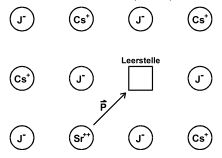
\includegraphics[width=6.5cm]{kristall.JPG}
 \caption{Dipol am Beispiel eines CsJ-Gitters mit Sr$^{2+}$-Kation \cite{V48}}
 \label{fig:aufbau}
 \end{subfigure}
 \begin{subfigure}{0.49\textwidth}
 \centering
 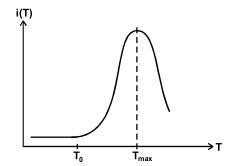
\includegraphics[width=6.5cm]{verlauf.JPG}
 \caption{Erwarteter Verlauf der Stromdichte gegenüber der Temperatur \cite{V48}}
 \label{fig:kurv}
 \end{subfigure}
 \end{figure}
 Bedingung für die Gültigkeit dieser Formel ist, dass die Zeit $t$ in der das E-Feld
 die Dipole ausrichtet groß gegenüber der Relaxationszeit $\tau(T)$ ist.
Durch schnelles Abkühlen dieses Zustandes gelingt es aufgrund des exponentiellen Anstiegs
der Relaxationszeit mit sinkender Temperatur die Dipolausrichtungen einzufrieren.
Eliminiert man nun zusätzlich die freien beweglichen Elektronen lässt sich durch das konstante Aufheizen der Probe mit der Heizrate $b=\frac{dT}{dt}=const$
ein Depolarisationsstrom erzeugen, welcher durch das Relaxieren der Dipole zurück in die räumliche Winkelverteilung entsteht.
Die Depolarisationsstromdichte $j(t)$ ergibt sich nach
\begin{equation}
  j(T) = y(T_\text{P}) p \frac{dN}{dt},
\label{eqn:strom}
\end{equation}
 mit $T_{P}$ als Polarisationstemperatur und $\frac{dN}{dt}$ als Zahl der pro Zeit und Volumeneinheit relaxierender Dipole.
 Der erwartete Verlauf der Depolarisationsstromdichte gegenüber der Temperatur aufgetragen ist in Abbildung \ref{fig:kurv} dargestellt.
Dieser Verlauf ergibt sich aufgrund der schnellen Abnahme der Relaxationszeit bis zum Maximum,
welches durch die sich steig verringernde Zahl der noch nicht relaxierten Dipole ergibt.
Der Faktor $\frac{dN}{dt}$ ist mit dem Proportionalitätsfaktor $\frac{1}{\tau}$ proportional zur Zahl
der noch pro Volumeneinheit orientierten Dipole.
\begin{equation}
\frac{dN}{dt}=\frac{N}{\tau}
\label{eqn:dif1}
\end{equation}
Die Lösung dieser Differentialgleichung
\begin{equation}
N=N_{\text{P}}\exp{-\frac{1}{b}\int_{T_{0}}^{T} \frac{dT'}{\tau(T')}}
\label{eqn:N}
\end{equation}
$N_{\text{P}}$ ist dabei die Dipolzahl zu Beginn des Aufheizens also bei der Temperatur $T_{0}$.
Das lässt sich nun mittel Gleichung \ref{eqn:dif1} in Formel \ref{eqn:strom} einsetzen und $\tau(T)$ durch Formel \ref{eqn:rel} ersetzen.
So erhält man für die Depolarisationsstromdichte
\begin{equation}
j(T)=\frac{p^{2}EN_{\text{P}}}{3kT_{\text{P}}\tau_{0}} \exp{\left(-\frac{1}{b\tau_{0}}\int_{T_{0}}^{T}\exp{-(\frac{W}{kT'})dT'}\right)}\exp{-\frac{W}{kT}}  .
\label{strom2}
\end{equation}
Um nun die gesuchte Potentialschwelle $W$ zu erhalten gibt es zwei Methoden.
Bei Methode 1 lässt sich im Anfangsbereich der Kurve der Depolarisationsstrom wegen
\begin{equation}
\int_{T_{0}}^{T'} \exp{(-\frac{W}{kT})}dT' \approx 0
\end{equation}
als
\begin{equation}
j(T) \approx \frac{p^{2}E N_{\text{P}}}{3k T_{\text{P}}\tau_{0}} \exp{-(\frac{W}{kT})}
\label{eqn:stmet1}
\end{equation}
nähern.
Für den Temperaturbereich indem diese Näherung gültig ist,
lässt sich W aus der Steigung der Ausgleichsgeraden die durch ein Diagramm gelegt wird, in dem
$\ln(j)$ gegen $\frac{1}{T}$ augetragen ist, berechnen.\\
Für eine genauere Bestimmung der gesuchten Werte wird Methode 2 angewandt bei der
die Schwellenenergie aus dem gesammten Kurvenverlauf bestimmt wird.
Hierzu wird für die Polarisation $P$ eine Differentialgleichung analog
zu Gleichung \ref{eqn:dif1} aufgestellt.
\begin{equation}
  \frac{dP}{dt}=\frac{P(t)}{\tau(T(t))}
\end{equation}
Durch die Integration des durch die Polarisation erzeugten Stromes $i(t)$
ergibt sich nun einen Ausdruck für
\begin{equation}
  \tau(T(t))=\frac{\int_{t(T)}^{\infty} i(t) dt}{i(t(T))} .
  \label{eqn:taum2}
\end{equation}
Da $t$ und $T$ über eine lineare Funktion zusammenhängen, lässt sich Gleichung \ref{eqn:taum2} auch als
\begin{equation}
  \tau(T)=\frac{\int_{T}^{\infty}i(T')dT'}{bi(T)}
\end{equation}
schreiben. Mit Formel \ref{eqn:rel} lässt sich nun ein Zusammenhang mit
der Potentialshwelle $W$ herstellen.
\begin{equation}
  \frac{W}{kT}=\frac{\int_{T}^{\infty}i(T')dT'}{bi(T)\tau_{0}}
  \label{eqn:strom2}
\end{equation}
Somit lässt sich nun $W$ bestimmen indem
\begin{equation}
  \ln \frac{\int_{T}^{T*}i(T')dT'}{i(T)}
\end{equation}
gegen $\frac{1}{T}$ aufgetragen wird. $T^*$ ist dabei eine beliebige Temperatur
bei der $i(T) \approx 0$ gilt.
  $\tau_{0}$ lässt sich bestimmen indem Gleichung \ref{eqn:strom2} nach $T$ differenziert wird und
 der Fall $T=T_{max}$ betrachtet wird für den die Ableitung gleich 0 ist.
 \begin{equation}
   \frac{\text{d}}{\text{d}T} \left( \frac{p^{2}EN_{\text{P}}}{3kT_{\text{P}}\tau_{0}} \exp{\left(-\frac{1}{b\tau_{0}}\int_{T_{0}}^{T}\exp{-(\frac{W}{kT'})dT'}\right)}\exp{-\frac{W}{kT}} \right)= \frac{W}{kT_{max}^{2}}-\frac{1}{b\tau_{0}}\exp{-\frac{W}{kT_{max}^2}}
 \end{equation}
 Mit der schon beshriebenen notwendigen Bedingung für Extremstellen
 lässt sich $\tau_{0}$ also als
 \begin{equation}
   \tau_{0}=\frac{kT_{max}^{2}}{Wb} \exp{-\frac{W}{kT_{max}^2}}
   \label{eqn:tau}
 \end{equation}
 ausdrücken.
